\chapter{Experimental Setup}\label{experimental_setup}

	This chapter explains the two similar experimental setups used to measure bubbles and discusses the resulting bubble images. First, the requirements for the setup are formally introduced in section \ref{requirements}, then the aquarium and the Aeolotron experimental setups that fulfill these requirements are explained in sections \ref{aquarium_setup} and \ref{aeolotron_setup}. Next, the acquired images are presented in section \ref{measurement_results}. Finally, the calibration setup is explained in section \ref{calibration_setup}  
	\section{Requirements}\label{requirements}
		In order to extend the previous work by \cite{Leonie}, we require that the developed method in this work fulfills the following criteria:
	\begin{itemize}
		\item \textbf{R1: Minimal distance to water surface}: This requirement defined the experimental setup. As shown in figures \ref{fig:aquarium_setup} and \ref{fig:aeolotron_setup}, lighting bubbles from below gives more freedom for the camera to be closer to the water surface. This is more apparent when the camera faces the surface with a certain angle. 
		\item \textbf{R2: Consistent image results}: Bubbles can look very different under different lighting conditions. For instance, bubbles might appear as dark disks or bright rings (chapter \ref{related_work}) depending on how they are lit. It is therefore required that the angle between the camera and the light source is always constant. This requirement guarantees a consistent pattern for bubbles across different water tanks.
		\item \textbf{R3: Images must contain all possibly retrievable information}. Simulation (figure \ref{subfig:bubble_simulation}) shows that bubbles are characterized by two peaks. Both of these – especially the upper, dimmer one – are required to be visible. This requires the camera to have a high signal-to-noise ratio and/or the light source to be very bright. 
	\end{itemize}	
	
	There is no unique setup that fulfills these requirements. So many parameters were chosen for practical reasons only. The following sections discuss two similar experimental setups that fulfill the requirements above. 
	
	
		
	\section{Aquarium Setup}\label{aquarium_setup}
		\begin{figure}
			\begin{subfigure}[t]{.5\textwidth}
				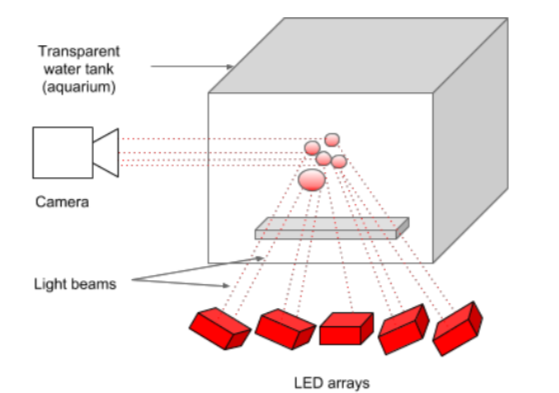
\includegraphics[scale=.6]{images/aquarium_setup.png}
				\caption{3D view.}
				\label{subfig:aquarium_setup_above}
			\end{subfigure}\hfill
			\begin{subfigure}[t]{.4\textwidth}
				\includegraphics[scale=.6]{images/aquarium_setup_above.png}
				\caption{View from above.}
			\end{subfigure}
			\caption{Experimental setup illustrating the $90^\circ$ angle between the light source (LED array) and the camera. Note how LEDs are oriented towards the camera's field of view to maximize the amount of light reaching the camera and therefore reduce noise.}
			\label{fig:aquarium_setup}
		\end{figure}			
		
		The goal of this setup was to capture bubble images that can be used to prototype the proposed algorithm. So the experiment was built in a transparent $1m \times 1m \times 1m$ water tank as shown in figure \ref{fig:aquarium_setup}. In order to satisfy requirements in section \ref{requirements}, parameters were set according to table \ref{tab:aquarium_param}. 
		 In this setup, most of the parameters could be changed such as lighting angle, camera and bubble concentration independently from each other. The obtained images are discussed in section \ref{measurement_results} and image analysis is discussed in chapter \ref{the_algorithm}.
		 
		 The setup consists of a transparent water tank (aquarium), one camera, a light source (LED arrays) and a bubble generator. 
		 
		 LED arrays were mounted underneath the water tank, and were oriented towards the camera's field of view to maximize the amount of light reaching the camera. As for the camera itself, it faces the light source at a $90^\circ$ angle. 
		 Seen from above, as shown in figure \ref{subfig:aquarium_setup_above}, the bubble generator lies right next to the light source. This way, it does not block any light from the LEDs but it is still close enough, such that bubbles within the camera's field of view are well lit. 
		
		We chose the Basler A1920 camera mainly because of its high signal-to-noise ratio, and therefore fulfilling requirement R3 given enough light. Its main drawback is its relatively low frame rate at the highest possible resolution, which makes bubble tracking more difficult, which in turn makes radius calibration more difficult (see section \ref{calibration_algorithm}). Compared to an available high-speed camera with comparable maximum resolution, (PCO Dimax, 1,2kHz at $2000 \times 2000$ resolution) the chosen camera also has a smaller sensor. This means that the magnification is higher and therefore smaller bubbles can be better detected ($50 \, \mu m/px$ vs $30 \, \mu m /px$). A 100 mm macro lens from Zeiss was used in this setup. The large focal length contributes to the large magnification factor of $30 \, \mu m /px$.
	
	Bubbles were produced by a bubble generator. Bubble radii therefore depend on the amount of air flowing through the bubble generator, measured in liter per minute or LPM. We acquired two sets of measurements, the first with a low bubble concentration, (1.8 LPM air flow), and the second with a much higher bubble concentration (3 LPM). 
		
		\begin{table}[h]
			\centering
		
			\begin{tabular}{|c|c|}
			\hline 
			Camera & Basler A1920-155um \\ 
			\hline 
			Focal length & Zeiss 100 mm macro \\ 
			\hline 
			F-number & 5,6 \\ 
			\hline 
			Exposure time & 100 $\mu s$ \\ 
			\hline 
			Gamma & 0,8 \\
			\hline
			Resolution [px] &1920 x 1200 \\
			\hline 
			Sensor size & 11.3 mm x 7.1 mm \\
			\hline 
			Magnification factor & $30 \, \mu m/px$ \\ 
			\hline 
			Framerate & 100 Hz \\ 
			\hline 
			Resulting field of view & 5,7cm x 3,6 cm \\
			\hline
			Bubble generator & FIAP profiO$_2$ Keramik\\			
			\hline
			Air flow & 1,8 LPM / 3 LPM \\ 
			\hline
			\end{tabular} 
			
			\caption{Parameters for aquarium setup}
			\label{tab:aquarium_param}

		\end{table}
		
	\section{Aeolotron Setup}\label{aeolotron_setup}
		The Aeolotron is an annular wind-wave facility with a diameter of about $10 \, m$ and a width of about $60 \, cm$. Typical water height is 1m. Four wind engines generate reference wind speeds of up to $17 \, m/s$, enough to generate breaking waves that can produce air bubbles. 
		
		The goal of this setup is to apply the knowledge gained from the aquarium setup to bubbles emerging from breaking waves, so the setup from the aquarium was reproduced at the Aeolotron, while keeping as many parameters unchanged as possible. Figure \ref{fig:aeolotron_setup} shows a schematic view of the wind facility as well as the experimental setup. 
		
		Similarly to the aquarium setup, the Aeolotron setup consisted of one camera, a light source and a bubble generator. 
		The light source was mounted underneath the Aeolotron and the camera was set with an $90^\circ$ relative to the light source. The bubble generator was laid at around 1 meter away from the light source (see \ref{subfig:aeolotron_setup_above}). A wind speed of $u_{10} = 8 m/s$ \footnote{$u_{10}$ refers to the wind speed at $10 \, m$ distance from the water surface. Turbine frequency was set at 15 Hz, which corresponds to $u_{10} = 8 m/s$ \citep{Bopp2018}.} was set. This wind speed is not high enough to generate breaking waves. However, it generated currents strong enough to ensure a random bubble distribution around the camera's field of view. Table \ref{tab:aeolotron_setup} summarizes the setup's parameters.
	
		\begin{table}
			\centering
		
			\begin{tabular}{|c|c|}
			\hline 
			Camera & Basler A1920-155um \\ 
			\hline 
			Focal length & Zeiss 100 mm macro\\ 
			\hline 
			F-number & 5,6 \\ 
			\hline 
			Exposure time & 130 $\mu s$ \\ 
			\hline 
			Gamma & 0,7 \\
			\hline
			Resolution [px] &1920 x 1200 \\
			\hline 
			Sensor size & 11.3 mm x 7.1 mm \\
			\hline 
			Magnification factor & 10 um/px \\ 
			\hline 
			Framerate & 100 Hz \\ 
			\hline 
			Resulting field of view & 1,9 cm x 1,2 cm \\
			\hline
			Bubble generator & FIAP profiO$_2$ Keramik\\			
			\hline
			Air flow & 1,8 LPM  \\ 
			\hline
			\end{tabular} 
			
			\caption{Parameters for Aeolotron setup}
			\label{tab:aeolotron_setup}

		\end{table}
		
		\begin{figure}[h]
			\centering
			\begin{subfigure}[t]{.3\linewidth}
				\centering
				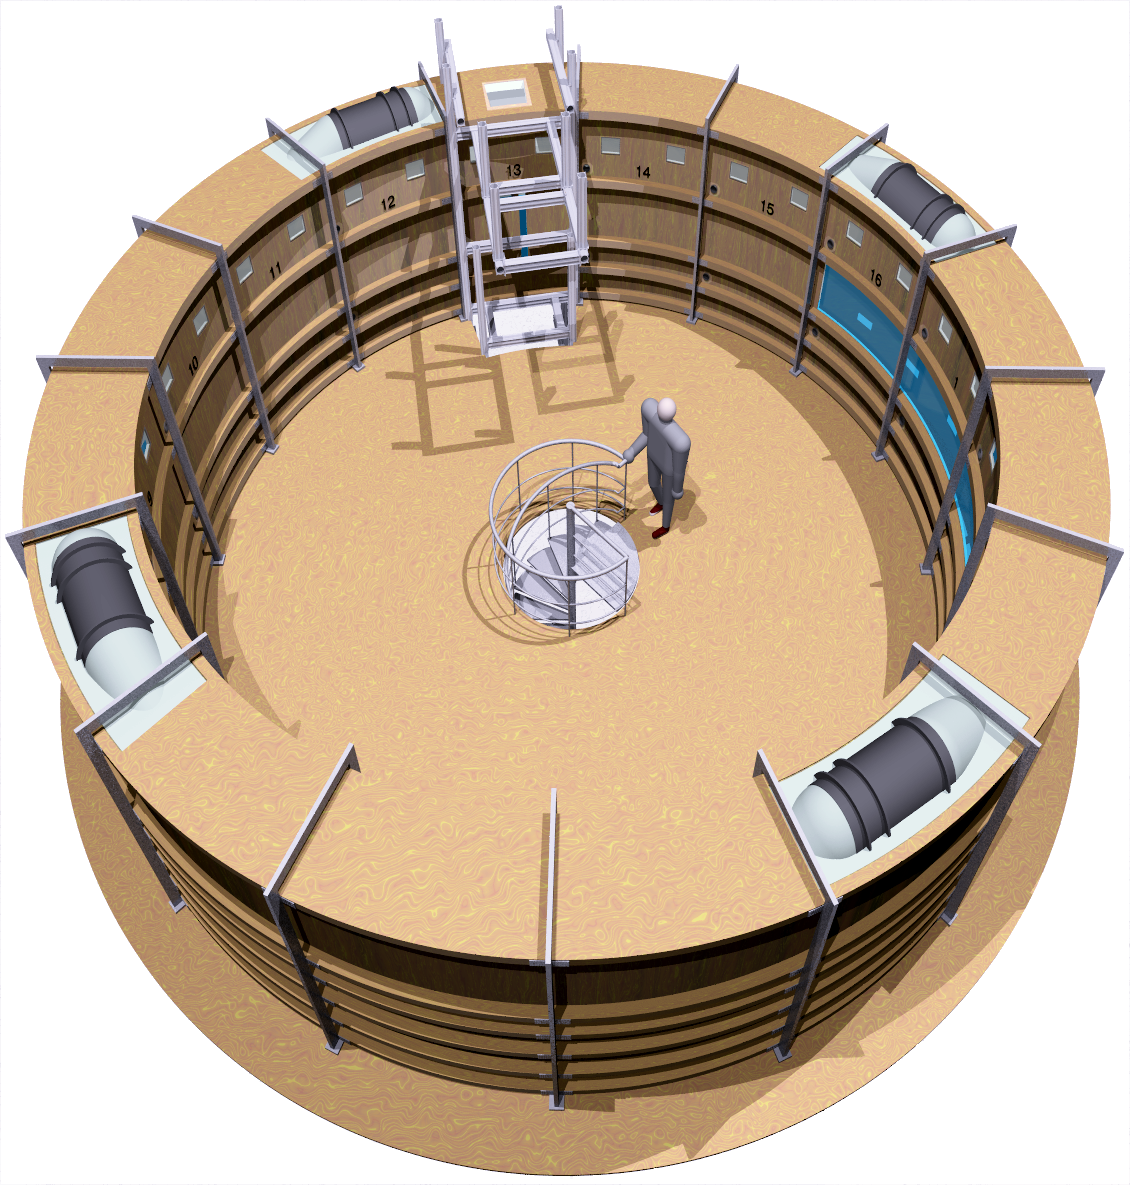
\includegraphics[scale=0.15]{images/aeolotron-gesamt.png}
				\caption{Aeolotron wind wave facility \citep{Krall2013}.}
			\end{subfigure}
			
			\begin{subfigure}[t]{.4\linewidth}		
				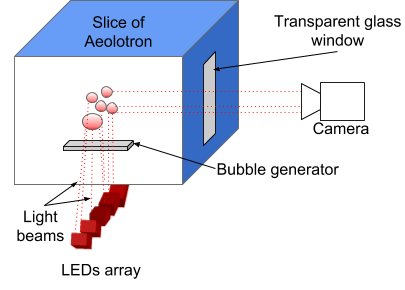
\includegraphics[scale=.5]{images/aeolotron_setup.png}
				\caption{Experimental setup.}
			\end{subfigure}\hfill%
			\begin{subfigure}[t]{.4\linewidth}		
				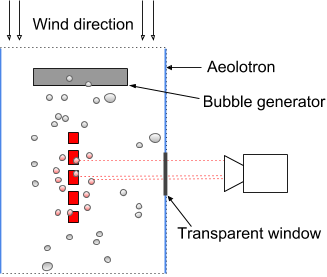
\includegraphics[scale=.5]{images/aeolotron_setup_above.png}
				\caption{Aeolotron from above.}
				\label{subfig:aeolotron_setup_above}
			\end{subfigure}
			
			\caption{Aeolotron facility and experimental setup.}
			\label{fig:aeolotron_setup}
		\end{figure}
	
		
		
	\section{Acquired Bubble Images}\label{measurement_results}
		\begin{figure}[h]			
			\begin{subfigure}[t]{.4\textwidth}
				\centering
				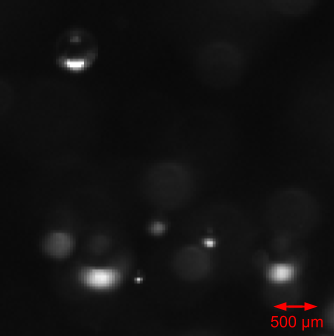
\includegraphics[scale=0.5]{images/aq_result_low_small_1.png}
				\caption{}
				\label{subfig:low_a}
			\end{subfigure}\hfill
			\begin{subfigure}[t]{.4\textwidth}
				\centering
				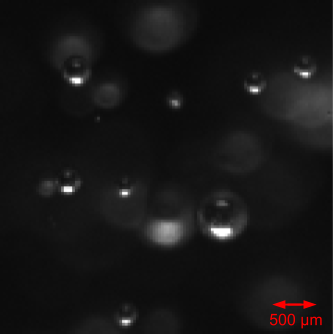
\includegraphics[scale=0.5]{images/aq_result_low_small_2.png}				
				\caption{}
				\label{subfig:low_b}				
			\end{subfigure}
			
			\begin{subfigure}[t]{.4\textwidth}
				\centering
				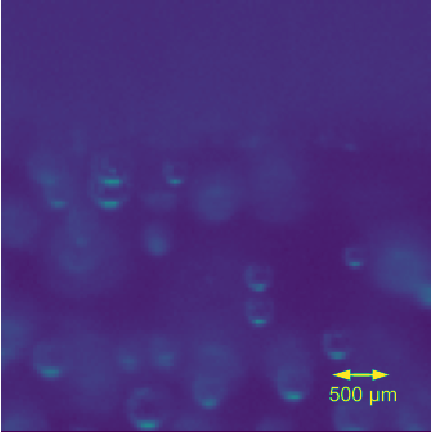
\includegraphics[scale=0.5]{images/aq_result_surf_small_1.png}				
				\caption{}
				\label{subfig:low_c}				
			\end{subfigure}\hfill
			\begin{subfigure}[t]{.4\textwidth}
				\centering
				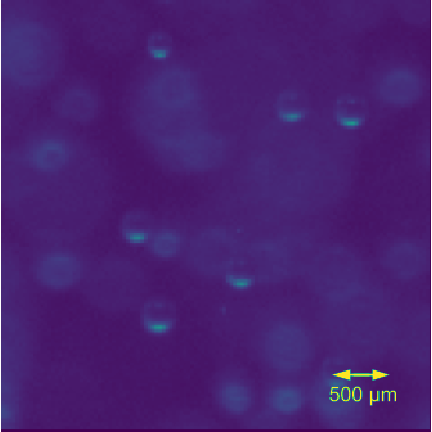
\includegraphics[scale=0.5]{images/aq_result_surf_small_2.png}
				\caption{}
				\label{subfig:low_d}				
			\end{subfigure}\hfill			
			\caption{Sample image captured with aquarium setup for a low bubble concentration for different camera setups. Note how bubbles are characterized by one bright peak at the bottom and one dimmer upper peak, as expected from simulation.}			
			\label{fig:aqauarium_result}
		\end{figure}
					
					
		\begin{figure}[h]
			\begin{subfigure}[t]{.4\textwidth}
				\centering
				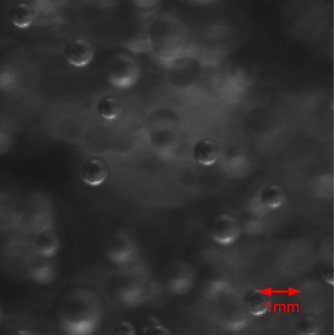
\includegraphics[scale=0.5]{images/aquarium_result_high_conc_1.png}
				\caption{}
				\label{subfig:aquarium_result_sat}
			\end{subfigure}\hfill
			\begin{subfigure}[t]{.4\textwidth}
				\centering
				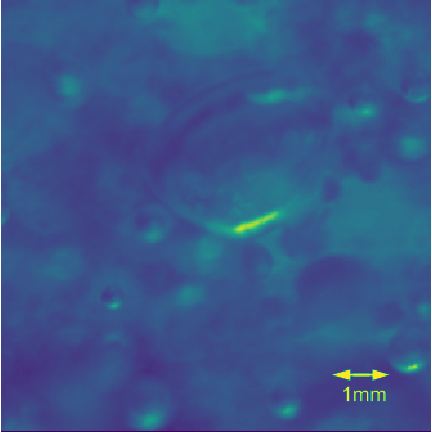
\includegraphics[scale=0.5]{images/aquarium_result_high_conc_2.png}
				\caption{}
				\label{subfig:too_large_bubble}
			\end{subfigure}\hfill		
			\caption{Sample images captured with aquarium setup for a high bubble concentration. The upper peak is not visible anymore. However, bubble curvatures are more recognizable, even for smaller bubbles}
			\label{fig:aquarium_result_high_conc}
		\end{figure}							
					
			\begin{figure}
				\begin{subfigure}[t]{.55\textwidth}
				\centering
				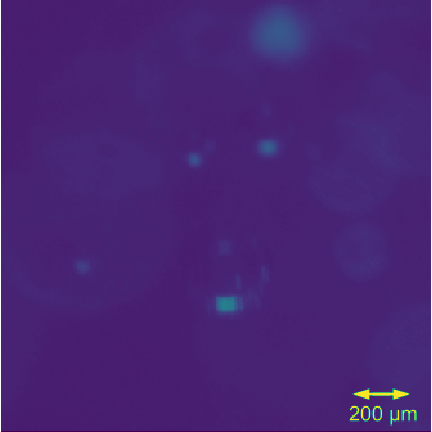
\includegraphics[scale=0.5]{images/aeolotron_result_small_1.png}
				\caption{}
				\label{subfig:aquarium_result_sat}
			\end{subfigure}\hfill
			\begin{subfigure}[t]{.55\textwidth}
				\centering
				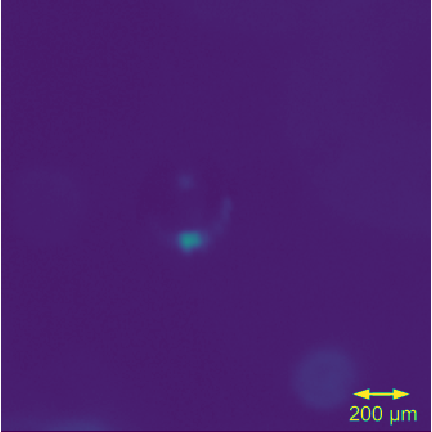
\includegraphics[scale=0.5]{images/aeolotron_result_small_2.png}
				\caption{}
			\end{subfigure}
				\caption{Image captured with Aeolotron setup. Bubbles were created by a bubble generator. Magnification is now larger than with the aquarium setup.}
								
				\label{fig:aeolotron_result}
			\end{figure}

			Figures \ref{fig:aqauarium_result} and \ref{fig:aquarium_result_high_conc} show images captured using a bubble generator with the aquarium setup. For low bubble concentrations, bubbles can be recognized by their characteristic bright lower peak. 
			However, when the concentration is very high (figure \ref{fig:aquarium_result_high_conc}) bubbles change dramatically. The curvature can be easily distinguished and scattered light from other bubbles gives bubbles a more circular shape. Also, the background is much brighter for a high bubble concentration. Figure \ref{subfig:too_large_bubble} shows a bubble so large that it lost its spherical shape. Such bubbles are too rare and will be classifier as background with no further considerations. 
			The exact bubble shape will be discussed further in chapter \ref{the_algorithm}.	Full size, raw measurements can be found in the appendix. 
	
	
	\section{Calibration}\label{calibration_setup}
		\subsection{Depth of Field}\label{sub:depth_of_field_setup}
			Since the measurement volume needs to be determined, it is not only necessary to detect bubbles in an image, but also to determine their depth, i.e. distance to the focal plane. With the experimental setup shown in figure \ref{fig:depth_of_field_setup}, bubbles can be trapped and moved along the depth axis. 
			
			Figure \ref{fig:depth_of_field_setup_result} shows images captured with this setup. Note how blurriness varies among images depending on the distance to the focal plane. In section \ref{calibration_algorithm} we discuss how to extract depth form these images. The setup is not perfectly stable, so resulting images were not perfectly aligned. As a workaround, additional images were captured with a different light source at each position to make other surrounding objects visible, e.g. armature of calibration device that can later on be used as reference objects to align images. 
			
			This calibration technique is practical, because only relative distances to the focal plane are needed for depth calibration. This is important because the goal of calibration is to determine the measurement volume only and not necessarily the absolute position of the bubbles to the camera. 
			
			
			\begin{SCfigure}
				\centering
				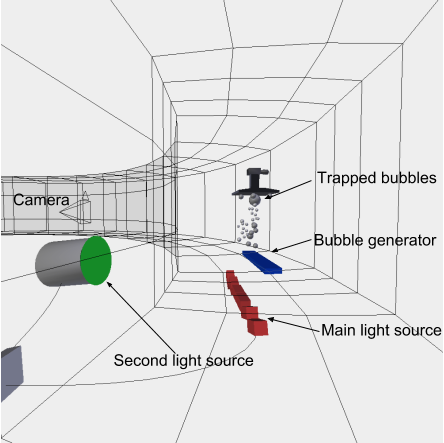
\includegraphics[scale=.5]{images/depth_of_field_setup.png}
				\caption{Setup for depth of field calibration. A high friction stick attached to a micrometer screw traps bubbles and moves them away from the focal plane.}
				\label{fig:depth_of_field_setup}
			\end{SCfigure}
			
			\begin{figure}
				\begin{subfigure}[b]{.55\textwidth}
					\centering
					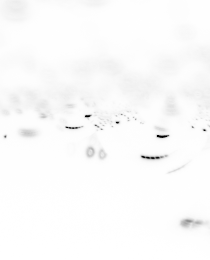
\includegraphics[scale=.5]{images/dof_calib_1.png}
					\caption{}
				\end{subfigure}%
				\begin{subfigure}[b]{.55\textwidth}
					\centering
					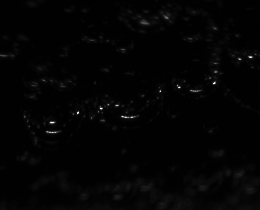
\includegraphics[scale=.5]{images/dof_calib_2.png}
					\caption{}
				\end{subfigure}
				
				\caption{Two images from depth of field calibration setup at different distances from focal plane.}								
				\label{fig:depth_of_field_setup_result}
			\end{figure}
			
			
		\subsection{Radius}\label{sub:radius_setup}
			Although simulation shows that the distance between the two dominant peaks in a bubble is proportional to the bubble radius, the real radius cannot be determined from measurement results alone (figure \ref{fig:aqauarium_result} and \ref{fig:aeolotron_result}). Therefore, lighting needs to be changed in such a way that the real radius, i.e. the whole bubble becomes measurable. In a similar way to the light field method \cite{MischlerDiss}, an additional light source and a mirror were mounted in order to light up bubbles from behind (figure \ref{fig:radius_calibration_setup}). Then, images were acquired at a frame rate of 200 FPS, where the second light source was turned on every second frame. Results are shown in figure \ref{fig:radius_calibration_setup_result}. In section \ref{calibration_algorithm} bubbles lit from below are identified with those lit from behind in order to estimate the proportionality factor between the real radius and the radius computed by the proposed algorithms. 
			

			\begin{SCfigure}
				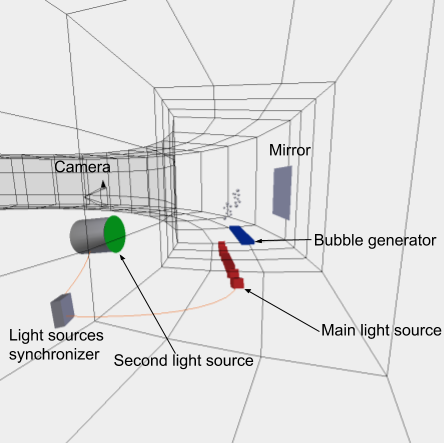
\includegraphics[scale=.5]{images/radius_setup_fancy.png}
				\caption{A view from inside the Aeolotron wind wave facility for radius calibration. The additional light source (green) is synchronized with the main light source (red).}
				\label{fig:radius_calibration_setup}
			\end{SCfigure}
			
			\begin{figure}
				\begin{subfigure}[b]{.55\textwidth}
					\centering
					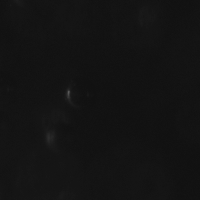
\includegraphics[scale=.7]{images/rad_calib_1.png}
					\caption{}
				\end{subfigure}
				\begin{subfigure}[b]{.55\textwidth}
					\centering
					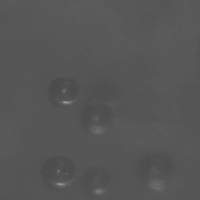
\includegraphics[scale=.7]{images/rad_calib_2.jpg}
					\caption{}
				\end{subfigure}
				\begin{subfigure}[b]{.55\textwidth}
					\centering
					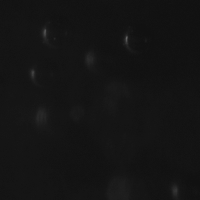
\includegraphics[scale=.7]{images/rad_calib_3.png}
					\caption{}
				\end{subfigure}
				\begin{subfigure}[b]{.55\textwidth}
					\centering
					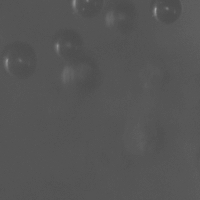
\includegraphics[scale=.7]{images/rad_calib_4.jpg}
					\caption{}
				\end{subfigure}
				
				\caption{Radius calibration images. (a) and (c) are lit from below. (b) and (d) are lit from below and from behind such that the real bubble radius becomes visible. }
				\label{fig:radius_calibration_setup_result}
			\end{figure}

































